% !TEX TS-program = pdflatex
\documentclass[letterpaper, 10pt, conference]{IEEEtran} %Especificación del tipo de documento
\IEEEoverridecommandlockouts %Este comando solo es necesario si se quiere usar el comando \thanks
\usepackage[spanish]{babel} %Paquete de manejo de idioma español
\usepackage[utf8]{inputenc} %Paquete para incluir caracteres con acentos
\usepackage{amsmath, amssymb, amsfonts} %Paquete para manejo de ecuaciones matemáticas, símbolos, etc.
\usepackage{graphicx} %Paquete para manejo de imágenes
\usepackage{xcolor} %Paquete para manejo de colores
\usepackage{hyperref} %Paquete para manejo de hipervínculos como enlaces de internet y enlaces directos del documento como en la tabla de contenido

\def \IEEEkeywordsname{Palabras Clave}
\def \IEEEproofname{Demostración}

\def \BibTeX{
	{\rm B\kern-0.05em{\sc i\kern-0.025em b}\kern-0.08em
	T\kern-0.1667em\lower0.7ex\hbox{E}\kern-0.125emX}
}

\title{Título del artículo \\
	{\footnotesize \textsuperscript{*}Nota: Los subtítulos no son captados en Xplore y no deberían ser usados}
	\thanks{Aquí se puede identificar la agencia de financiación aplicable. Si no hay ninguna, se puede eliminar esto.}
}

\author{
	\IEEEauthorblockN{1\textsuperscript{er} Nombre y Apellido}
	\IEEEauthorblockA{\textit{Nombre del Depto. de la Organización} \\
		\textit{Nombre de la Organización} \\
		País, Ciudad \\
		\href{John.A.Doe@ieee.org}{Correo Electrónico}
	}
	\and
	\IEEEauthorblockN{2\textsuperscript{do} Nombre y Apellido}
	\IEEEauthorblockA{\textit{Nombre del Depto. de la Organización} \\
		\textit{Nombre de la Organización} \\
		País, Ciudad \\
		\href{John.A.Doe@ieee.org}{Correo Electrónico}
	}
	\and
	\IEEEauthorblockN{3\textsuperscript{er} Nombre y Apellido}
	\IEEEauthorblockA{\textit{Nombre del Depto. de la Organización} \\
		\textit{Nombre de la Organización} \\
		País, Ciudad \\
		\href{John.A.Doe@ieee.org}{Correo Electrónico}
	}
	\and
	\IEEEauthorblockN{4\textsuperscript{to} Nombre y Apellido}
	\IEEEauthorblockA{\textit{Nombre del Depto. de la Organización} \\
		\textit{Nombre de la Organización} \\
		País, Ciudad \\
		\href{John.A.Doe@ieee.org}{Correo Electrónico}
	}
	\and
	\IEEEauthorblockN{5\textsuperscript{to} Nombre y Apellido}
	\IEEEauthorblockA{\textit{Nombre del Depto. de la Organización} \\
		\textit{Nombre de la Organización} \\
		País, Ciudad \\
		\href{John.A.Doe@ieee.org}{Correo Electrónico}
	}
	\and
	\IEEEauthorblockN{6\textsuperscript{to} Nombre y Apellido}
	\IEEEauthorblockA{\textit{Nombre del Depto. de la Organización} \\
		\textit{Nombre de la Organización} \\
		País, Ciudad \\
		\href{John.A.Doe@ieee.org}{Correo Electrónico}
	}
}

\begin{document}
	\maketitle
	
	\begin{abstract}
		Este documento es un ejemplo del formato definido por las normas IEEE para escribir artículos representativos de un proyecto realizado. Los autores deben seguir las instrucciones, incluyendo formato y tamaño de papel para mantener el estándar de publicación. Este documento puede interpretarse como un conjunto de instrucciones para escribir el artículo o como una plantilla para hacerlo. Como se habrá notado, esta primera sección es para generar un resumen muy corto y a alta escala del alcance y resultados del proyecto. IMPORTANTE: No usar símbolos, caracteres especiales, notas de pie de página ni ecuaciones matemáticas en el título o resumen del documento.
	\end{abstract}
	
	\begin{IEEEkeywords}
		IEEE, componente, formato, estilo, insertar, referencias
	\end{IEEEkeywords}
	
	\section{Introducción} \label{seccionIntroduccion}
	Este documento es un modelo que cuenta con instrucciones para {\LaTeX}, es importante observar los límites de página del tipo de documento para conferencias.
	
	La IEEE \emph{(Instituto de Ingenieros Eléctricos y Electrónicos)} es una organización sin ánimo de lucro cuyo objetivo es promover la creatividad, desarrollo, integración, aplicabilidad y el compartir de los avances en tecnologías de información y ciencias en general para el beneficio de la humanidad y de los mismos profesionales \cite{referenciaBibliografica1}, además, es una de las organizaciones más importantes en la creación de estándares a nivel mundial, y en particular, tiene definidas unas normas de caracter universal para la construcción de artículos científicos, reportes de resultados de proyectos y de investigación, utilizados ampliamente en ingeniería y ciencias, como parte de la etapa de formación académica en universidades, actividades de investigación, etc.
	
	El propósito con el cual se revisa y se mejora esta plantilla, es facilitar a los usuarios la obtención de este recurso y su usabilidad al momento de construir su artículo, de forma que no tengan que preocuparse por ajustar márgenes, enumeraciones de secciones, formato de los textos y otros aspectos directamente relacionados al estilo del documento o formato de los textos.
	
	El archivo de clase IEEEtran.cls, el cual está fuera del archivo principal Documento.tex, es la base sobre la cual se aplica el formato y normas fundamentales IEEE en el archivo Documento.pdf generado sobre el archivo principal Documento.tex, dicho archivo de clase ha sido implementado y actualizado por Gerry Murray, Silvano Balemi, Jon Dixon, Peter Nuchter, Juergen von Hagen y Michael Shell, este último, es actual responsable del mantenimiento de este archivo de clase para futuras modificaciones y actualizaciones \cite{referenciaBibliografica2}.
	
	A pesar de las constantes actualizaciones de normas IEEE en casi cualquier industria, se tiene un inconveniente respecto al tamaño máximo que pueden ocupar en el documento los elementos gráficos como imágenes, gráficos estadísticos, tablas, mapas, etc., debido a que las normas IEEE en su estilo de documento toma en cuenta el uso de dos columnas de texto y esto puede dificultar la legibilidad de dichos elementos gráficos para los lectores, a partir de esta observación, se tiene de forma alternativa esta misma plantilla pero con texto a solo una columna de forma que se mantengan las demás normas del estilo del documento y permitir que estos elementos gráficos puedan ocupar de ancho la mayor parte de la página y mejorar su legibilidad a los lectores.
	
	\section{Facilidad de Uso} \label{seccionFacilidadDeUso}
	\subsection{Acceso Libre a la Plantilla} \label{subseccionAccesoLibreALaPlantilla}
	Para reutilizar esta plantilla, esta versión en español a dos columnas se puede encontrar para su posterior edición disponible en Overleaf en \href{https://es.overleaf.com/read/dntrzbbwdxkv}{https://es.overleaf.com/read/dntrzbbwdxkv} o de forma local con el IDE TexStudio disponible en el repositorio de Github en \href{https://github.com/mamurciac/DocumentsTemplates_PublicVersion/tree/main/IEEE%20Report%20%5BSpanish%20with%20Double%20Column%5D}{https://github.com/mamurciac/DocumentsTemplates\_ PublicVersion/tree/main/IEEE\%20Report\%20\%5BSpanish\% 20with\%20Double\%20Column\%5D} para su posterior descarga y edición.
	
	También se tienen disponibles las siguientes versiones (según el idioma y número de columnas):
	\begin{itemize}
		\item Español a una sola columna, disponible en Overleaf en \href{https://es.overleaf.com/read/rtrmjjvkhszt}{https://es.overleaf.com/read/rtrmjjvkhszt} o de forma local en el repositorio de Github en \href{https://github.com/mamurciac/DocumentsTemplates_PublicVersion/tree/main/IEEE%20Report%20%5BSpanish%20with%20Single%20Column%5D}{https://github.com/mamurciac/DocumentsTemplates\_ PublicVersion/tree/main/IEEE\%20Report\%20\%5BSpanish\% 20with\%20Single\%20Column\%5D}.
		\item Inglés a dos columnas, disponible en Overleaf en \href{https://es.overleaf.com/read/yvwjymdknjjm}{https://es.overleaf.com/read/yvwjymdknjjm} o de forma local en el repositorio de Github en \href{https://github.com/mamurciac/DocumentsTemplates_PublicVersion/tree/main/IEEE%20Report%20%5BEnglish%20with%20Double%20Column%5D}{https://github.com/mamurciac/DocumentsTemplates\_ PublicVersion/tree/main/IEEE\%20Report\%20\%5BEnglish\% 20with\%20Double\%20Column\%5D}.
		\item Inglés a una sola columna, disponible en Overleaf en \href{https://es.overleaf.com/read/gvyvqvsdkzfy}{https://es.overleaf.com/read/gvyvqvsdkzfy} o de forma local en el repositorio de Github en \href{https://github.com/mamurciac/DocumentsTemplates_PublicVersion/tree/main/IEEE%20Report%20%5BEnglish%20with%20Single%20Column%5D}{https://github.com/mamurciac/DocumentsTemplates\_ PublicVersion/tree/main/IEEE\%20Report\%20\%5BEnglish\% 20with\%20Single\%20Column\%5D}.
	\end{itemize}
	
	\subsection{Mantenimiento de Integridad de las Especificaciones} \label{subseccionMantenimientoDeIntegridadDeLasEspecificaciones}
	El archivo de clase IEEEtran.cls se usa para dar formato al papel y estilo al texto; se preescriben todos los márgenes, anchos de columna, espacios de línea y fuentes de texto; se recomienda no alterarlos. Se podrá notar algunas peculiaridades, por ejemplo, el margen de encabezado mide proporcionalmente más de lo habitual, esta medición y otras son deliberadas, utilizando especificaciones que anticipan su trabajo como una parte de todo el proceso, y no como un documento independiente. Se pide no revisar ninguna de las designaciones actuales.
	
	\section{Preparación del Documento Antes de Aplicar Formato} \label{seccionPreparacionDelDocumentoAntesDeAplicarFormato}
	Antes de comenzar a dar formato al trabajo, se recomienda primero escribir y guardar el contenido como un archivo de texto separado, completar todo el contenido y la edición organizacional antes de aplicar formato. También se recomienda tener en cuenta las secciones \ref{subseccionAbreviaturasYAcronimos} y \ref{subseccionAlgunosErroresComunes} a continuación para obtener más información sobre revisión, ortografía y gramática.
	
	Se pide mantener los archivos de texto y gráficos separados hasta que el texto haya sido formateado y tenga el estilo apropiado, además de no enumerar los encabezados de texto pues {\LaTeX} lo hará automáticamente.
	
	\subsection{Abreviaturas y Acrónimos} \label{subseccionAbreviaturasYAcronimos}
	Se recomienda definir abreviaturas y acrónimos la primera vez que se usan en el texto, incluso después de que se hayan definido en el resumen. No es necesario definir abreviaturas como IEEE, SI, MKS, CGS, ac, dc o rms, y se pide no usar abreviaturas en el título o encabezados a menos que sean inevitables.
	
	\subsection{Unidades} \label{subseccionUnidades}
	\begin{itemize}
		\item Se recomienda usar las unidades del SI \emph{(Sistema Internacional)}, que en particular contienen las unidades MKS \emph{(Metro, kilogramo y segundo)}, o CGS \emph{(Sistema Cegesimal)} como unidades de medida primarias, se recomienda especialmente las unidades del SI.
		\item Las unidades en inglés se pueden usar como unidades de medida secundarias (entre paréntesis) aunque una excepción sería el uso de unidades inglesas como identificadores en el comercio, como la ``unidad de disco de 3.5 pulgadas''.
		\item No es recomendable combinar unidades del SI y CGS, como corriente en amperios y campo magnético en oersteds, esto a menudo conduce a la confusión porque las ecuaciones no se equilibran dimensionalmente. Si se debe usar unidades mixtas, se debe indicar claramente las unidades para cada cantidad que usa en una ecuación.
		\item No se debe mezclar deletreado completo con abreviaciones de unidades, por ejemplo, se puede usar ``Wb/m\textsuperscript{2}'' o ``webers por metro cuadrado'', pero no ``webers/m\textsuperscript{2}'', sin embargo, se pueden deletrear las unidades cuando aparecen en el texto, por ejemplo, es recomendable mencionar: ``. . . algunos henrys'', pero no ``. . . algunos H''.
		\item Se recomienda usar un cero antes de los puntos decimales, por ejemplo ``0.25'' pero no ``.25'', y también se recomienda usar ``cm\textsuperscript{3}'', en vez de ``cc'' para unidades de volumen.
	\end{itemize}
	
	\subsection{Ecuaciones} \label{subseccionEcuaciones}
	Se recomienda enumerar las ecuaciones numéricas consecutivamente. Para hacer las ecuaciones más compactas, se puede usar las barras (~/~), la función exponencial, o exponentes apropiados.
	
	Se recomienda poner en cursiva los símbolos en alfabeto romano para cantidades y variables, pero no los símbolos en alfabeto griego, también se recomienda usar un guión largo en lugar de un guión para un signo menos. 
	
	El siguiente elemento es un ejemplo de una ecuación:
	\begin{equation}
		a + b = \gamma
		\label{ejemploDeEcuacion}
	\end{equation}
	
	Para reconocimiento de variables y posiblemente algunas constantes poco conocidas, se recomienda asegurarse de que los símbolos en cada ecuación se hayan definido antes o inmediatamente después de la ecuación.
	
	Al momento de mencionar ecuaciones en el texto, es decir cuando forman parte de una oración, se recomienda usar ``\eqref{ejemploDeEcuacion}'', pero no ``Ec.~\eqref{ejemploDeEcuacion}'' ni ``ecuación \eqref{ejemploDeEcuacion}'', excepto al comienzo de una frase, por ejemplo, ``Ecuación \eqref{ejemploDeEcuacion} es . . .''.
	
	\subsection{Avisos Específicos de {\LaTeX}} \label{subseccionAvisosEspecificosDeLatex}
	Se pide usar referencias cruzadas ``suaves'' (e.g., \verb|\eqref{ejemploDeEcuacion}|) en lugar de referencias ``difíciles'' (e.g., \verb|(1)|), esto permitirá combinar secciones, agregar ecuaciones o cambiar el orden de las figuras o citas sin tener que pasar por el archivo línea por línea y sin mezclar referencias de unos elementos con otros; por ejemplo, para evitar mezclar referencias de figuras con referencias de tablas o incluso referencias de secciones que forman parte de la estructura del documento.
	
	Se recomienda no usar el ambiente de ecuaciones \verb|{eqnarray}|, sino usar los ambientes \verb|{align}| o \verb|{IEEEeqnarray}| en su lugar, esto se pide porque el ambiente \verb|{eqnarray}| deja espacios antiestéticos alrededor de los símbolos de relación y de algunos otros símbolos.
	
	Se pide notar que el ambiente \verb|{subequations}| en {\LaTeX} incrementará el contador de ecuaciones principal, incluso cuando no se muestren números de ecuaciones; si se olvida esto, se puede escribir un artículo en el que los números de ecuación salten de (17) a (20) por ejemplo, indicando posibles ecuaciones faltantes o fallas en la enumeración de estos elementos.
	
	{\BibTeX} no funciona por arte de magia, no obtiene los datos biblográficos de la nada sino de archivos .bib. Si se usa {\BibTeX} para producir una bibliografía, esta se debe enviar por medio de archivos .bib.
	
	{\LaTeX} no puede leer la mente, si se asigna la misma etiqueta a una subsección y a una tabla, se podrá encontrar que por ejemplo la Tabla I ha sido referenciada como Tabla IV-referenciaBibliografica3.
	
	{\LaTeX} no tiene habilidades precognitivas, si se pone un comando \verb|\label| antes del comando que actualiza el contador que se supone que debe estar usando, la etiqueta recogerá el último contador para ser referenciado en su lugar; en particular, un comando \verb|\label| no debería ir antes del título de una figura o una tabla.
	
	Se pide no usar el comando \verb|\nonumber| dentro del ambiente \verb|{array}|, esto no detendrá los números de ecuación dentro del comando \verb|{array}| (No habrá ninguno de todos modos) y se podría detener en un número de ecuación no deseado en la ecuación circundante.
	
	\subsection{Algunos Errores Comunes} \label{subseccionAlgunosErroresComunes}
	\begin{itemize}
		\item La palabra ``datos'' está en plural, no en singular.
		\item El subíndice para la permeabilidad del vacío $\mu_{0}$, y otras constantes científicas comunes, es cero con formato de subíndice, no una letra minúscula ``o''.
		\item En inglés americano, las comas, los puntos y comas, las preguntas y los signos de exclamación se encierran entre comillas solo cuando se cita un pensamiento o nombre completo, como un título o una cita completa. Cuando se utilizan comillas, en lugar de una fuente en negrita o cursiva para resaltar una palabra o frase, la puntuación debe aparecer fuera de las comillas. Una frase o declaración entre paréntesis al final de una frase se puntúa fuera del paréntesis de cierre (como este). (Una oración entre paréntesis se puntúa dentro de los paréntesis.)
		\item Un gráfico dentro de un gráfico es un ``recuadro''.
		\item No usar la palabra ``esencialmente'' para referirse a ``aproximadamente'' o ``efectivamente''.
		\item En el título del trabajo, si las palabras ``que usa'' pueden reemplazar con precisión la palabra ``usar'', se escribe en mayúscula la ``u''; si no, se manteniene la palabra en minúscula.
		\item Se recomienda ser consciente de los diferentes significados de las palabras cuasihomófonas ``afecto'' y ``efecto'', ``complemento'' y ``cumplimiento'', ``principal'' y ``principio''.
		\item No confundir ``implicar'' e ``inferir''.
		\item No hay un punto después de la palabra ``et'' en abreviación latina ``et al.'', esta expresión latina sin abreviar es \emph{``et alii''} que significa ``y otros'' en español.
		\item La expresión latina ``i.e.'' sin abreviar es \emph{``id est''} que significa ``es decir'' en español.
		\item La expresión latina ``e.g.'' sin abreviar es \emph{``exempli gratia''} que significa ``por ejemplo'' en español.
	\end{itemize}

	Un excelente manual de estilo para escritores científicos está en \cite{referenciaBibliografica3}.
	
	\subsection{Autores y Afiliaciones} \label{subseccionAutoresYAfiliaciones}
	\textbf{El archivo de clase está diseñado para, pero no limitado a seis autores,} se requiere de mínimo un autor para todos los artículos de conferencia. Los nombres de los autores se deben enumerar comenzando de izquierda a derecha y luego pasando a la siguiente línea, esta es la secuencia de autores que se utilizará en citas futuras y servicios de indexación, los nombres no deben aparecer en columnas ni agruparse por afiliación, además, se recomienda mantener las afiliaciones tan breves como sea posible (por ejemplo, no diferenciar entre los departamentos de la misma organización).
	
	\subsection{Identificación de Encabezados} \label{subseccionIdentificacionDeEncabezados}
	Los encabezados son recursos organizativos que guían al lector a través del trabajo. Hay dos tipos de encabezados: de componente y de texto.
	
	Los encabezados de componentes identifican los diferentes componentes del trabajo y no están subordinados por temas entre sí. Los ejemplos incluyen Agradecimientos y Referencias, y para estos, el estilo correcto para usar es ``Encabezado 5''. Se recomienda usar ``título de figura'' para los títulos de figuras, y ``encabezado de tabla'' para los títulos de tabla. Los encabezados iniciales, como ``Resumen'', requieren que se aplique un estilo (en este caso, cursiva) además del estilo proporcionado por el menú desplegable para diferenciar el encabezado del texto.
	
	Los encabezados de texto organizan los temas sobre una base relacional y jerárquica; por ejemplo, el título del trabajo es el encabezado principal del texto porque todo el material posterior se relaciona y elabora sobre este tema. Si hay dos o más subtemas, se debe utilizar el encabezado de nivel siguiente (con números romanos en mayúscula) y, por el contrario, si no hay al menos dos subtemas, no se debe introducir subtítulos.
	
	\subsection{Figuras y Tablas} \label{subseccionFigurasYTablas}
	\paragraph{Ubicación de Figuras y Tablas} Se recomienda ubicar figuras y tablas en la parte superior e inferior de las columnas, además de evitar ubicarlas en medio de las columnas. Las figuras grandes pueden abarcar ambas columnas.
	
	Los títulos de las figuras deben estar debajo de las figuras, los encabezados de las tablas deben aparecer sobre las tablas, se recomienda insertar figuras y tablas después de que se citan en el texto. Se puede usar la abreviatura ``Fig.~\ref{ejemploDeFigura}'', incluso al comienzo de una oración.
	
	\begin{table}[htbp]
		\caption{Estilo de tipo de tabla}
		\begin{center}
			\begin{tabular}{|c|c|c|c|}
				\hline
				\textbf{Encabezado} & \multicolumn{3}{|c|}{\textbf{Encabezado de columna de la tabla}} \\
				\cline{2-4}
				\textbf{de la tabla} & \textbf{\textit{Subencabezado}} & \textbf{\textit{Subencabezado}} & \textbf{\textit{Subencabezado}} \\
				 & \textbf{\textit{de columna}} & \textbf{\textit{de columna}} & \textbf{\textit{de columna}} \\
				\hline
				Texto & Más texto$^{\mathrm{a}}$ & & \\
				\hline
				\multicolumn{4}{l}{$^{\mathrm{a}}$Ejemplo de nota al pie de tabla.}
			\end{tabular}
			\label{ejemploDeTabla}
		\end{center}
	\end{table}
	
	\begin{figure}[htbp]
		\centerline{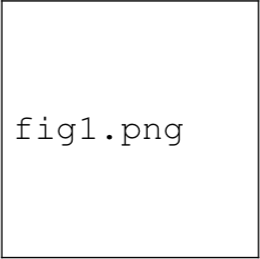
\includegraphics{Figuras/Figura1.png}}
		\caption{Ejemplo de un título de figura.}
		\label{ejemploDeFigura}
	\end{figure}
	
	\paragraph{Etiquetas de Figuras} Se recomienda usar letra Times New Roman de 8 puntos para etiquetas de figuras, Se puede usar palabras en lugar de símbolos o abreviaturas al escribir etiquetas de eje de figura para evitar confundir al lector; por ejemplo, escribir la cantidad ``Magnetización'', o ``Magnetización, M'', no solo ``M''. Si se incluyen unidades en la etiqueta, se deben presentar entre paréntesis. No se debe etiquetar los ejes solamente con las unidades; por ejemplo, se puede escribir ``Magnetización (A/m)'' o ``Magnetización \{Am\textsuperscript{-1}\}'', no solo ``A/m'', además, se recomienda no etiquetar los ejes con una proporción de cantidades y unidades, por ejemplo, escribir ``Temperatura (K)'', no ``Temperatura/K''.
	
	\section*{Reconocimientos} \label{seccionReconocimientos}
	Se recomienda evitar la expresión rígida ``uno de nosotros (R. B. G.) gracias $\ldots$'', en cambio, se puede usar ``R. B. G. gracias $\ldots$''. Se pide colocar los reconocimientos del patrocinador en la nota al pie sin enumerar, en la parte inferior de la primera página.
	
	\section*{Inclusión de Citas y Referencias en el Texto} \label{seccionInclusionDeCitasYReferenciasEnElTexto}
	Se pide enumerar las citas consecutivamente entre paréntesis \cite{referenciaBibliografica4}, La puntuación de oración sigue al paréntesis \cite{referenciaBibliografica5}. Se pide indicar simplemente el número de referencia, como en \cite{referenciaBibliografica6}--- en vez de ``Ref. \cite{referenciaBibliografica6}'' ni ``referencia \cite{referenciaBibliografica6}'' excepto al comienzo de una frase, por ejemplo, ``Referencia \cite{referenciaBibliografica6} fue el primer $\ldots$''.
	
	Se pide enumerar las notas al pie por separado en superíndices, colocar la nota al pie actual en la parte inferior de la columna en la que se citó. Se recomienda no poner notas al pie en el resumen o en la lista de referencias, ni usar letras para las notas al pie de tabla.
	
	A menos que haya seis autores o más, indicar los nombres de todos los autores sin excepción; se pide no usar ``et al.'' para omitir a autores faltantes de indicar. Los documentos que no se han publicado, incluso si se han enviado para su publicación, deben citarse como ``inéditos'' \cite{referenciaBibliografica7}, los trabajos que han sido aceptados para publicación deben citarse como ``en prensa'' \cite{referenciaBibliografica8}.
	
	Se debe escribir en mayúscula solo la primera palabra en un título de un documento, excepto los nombres propios y símbolos de los elementos.
	
	Para los trabajos publicados en revistas de traducción, se pide ingresar primero la cita en inglés, seguida de la cita en el idioma extranjero original \cite{referenciaBibliografica9}.
	
	\section*{Construcción de Referencias Bibliográficas} \label{seccionConstruccionDeReferenciasBibliograficas}
	En todo artículo de investigación, reporte de resultados de un proyecto, entre otros, se debe hacer uso ético, responsable y legítimo de la información necesaria y obtenida de cualquier recurso bibliográfico. Al incluir las referencias bibliográficas, se identifican las ideas e información de obras de otros autores además de dar el reconocimiento a ellos por la información extraída en esos recursos que aportan directamente en la construcción del artículo o reporte \cite{referenciaBibliografica10}.
	
	Al indicar las referencias bibliográficas, esto se debe hacer de forma estructurada, es decir, hay un estándar definido por IEEE, así como en APA \emph{(Asociación Americana de Psicología)}, ICONTEC \emph{(Instituto Colombiano de Normas Técnicas)} o ACM \emph{(Asociación de Maquinaria Computacional)} para redactar las referencias bibliográficas y así identificar cada recurso bibliográfico utilizado a partir de atributos como nombres de autores, título de la obra, país de elaboración, fechas de publicación, instituciones o empresas, etc.
	
	A continuación, se indica la estructura para redactar referencias bibliográficas a partir de normas IEEE, según el tipo de recurso o fuente:
	\begin{itemize}
		\item \textbf{\emph{Libro:}} Iniciales y Apellido(s) del(os) autor(es), \textit{Título del libro en letra cursiva}. Edición. Lugar de publicación: Editorial, Año de publicación.
		\item \textbf{\emph{Tesis de pregrado, magister o doctorado:}} Iniciales y Apellido(s) del(os) autor(es), ``Título de la tesis o proyecto'', Clase de documento (tesis doctoral, trabajo de fin de magister, etc.), Departamento, Institución académica (abreviada), Ciudad, Estado abreviado, Año.
		\item \textbf{\emph{Artículo de revista:}} Iniciales y Apellido(s) del(os) autor(es), ``Título del artículo'', \textit{Título abreviado de la revista en cursiva}, volumen (abreviado vol.), número abreviado (no.) páginas (abreviado pp.), Mes y Año.
		\item \textbf{\emph{Apuntes de clases:}} Iniciales y Apellido(s) del(os) autor(es) (si corresponde), ``Título de los apuntes o materia'', Notas de clase para Código de la asignatura, Departamento, Institución o Universidad, época/semestre y año.
		\item \textbf{\emph{De la web:}} Iniciales y Apellido(s) del(os) autor(es), Fecha de publicación en formato (año, mes y día). Título (edición) [Tipo de medio, generalmente En línea]. Dieponible en: Url/Enlace.
	\end{itemize}
	
	A continuación, se muestran ejemplos de referencias bibliográficas con normas IEEE:
	\begin{itemize}
		\item \textbf{\emph{Ejemplo de referencia IEEE de un libro:}} R. G. Gallager. \textit{Principles of Digital Communication}. Nueva York: Cambridge University Press, 2008.
		\item \textbf{\emph{Ejemplo de referencia IEEE de una tesis:}} H. Zhang, ``Delay-insensitive networks'', Tesis de magister, Universidad de Waterloo, Waterloo, ON, Canadá, 1997.
		\item \textbf{\emph{Ejemplo de referencia IEEE de un artículo de revista:}} G. Liu, K. Y. Lee, y H. F. Jordan, ``TDM and TWDM de Brujin networks and suffflenets for optical communications'', \textit{IEEE Transactions on Computers}, vol. 46, pp. 695-701, Junio 1997.
		\item \textbf{\emph{Ejemplo de referencia IEEE de apuntes de clase:}} ``Signal integrity and interconnects for high-speed applications'', notas de clase para ECE497-JS, Departamento de Ingeniería Eléctrica y de Computación, Universidad de Illinois sede Urbana-Champaign, segundo semestre 1997.
		\item \textbf{\emph{Ejemplo de referencia IEEE de la web:}} J. Jones. (1991, Mayo 10). Networks (2da ed.) [En línea]. Disponible en: \href{http://www.atm.com}{http://www.atm.com}.
	\end{itemize}
	
	\begin{thebibliography}{00}
		\bibitem{referenciaBibliografica1} (2021, Diciembre 29). Institute of Electrical and Electronics Engineers [En línea]. Disponible en: \href{https://es.wikipedia.org/wiki/Institute_of_Electrical_and_Electronics_Engineers}{https://es.wikipedia.org/wiki/Institute\_of\_Electrical\_and\_Electronics\_ Engineers}.
		\bibitem{referenciaBibliografica2} (2015, Agosto 26). CTAN Comprehensive TEX Archive Network [En línea]. Disponible en: \href{https://www.ctan.org/tex-archive/macros/latex/contrib/IEEEtran/}{https://www.ctan.org/tex-archive/macros/latex/contrib/IEEEtran/}.
		\bibitem{referenciaBibliografica3} M. Young, The Technical Writer's Handbook. Mill Valley, CA: University Science, 1989.
		\bibitem{referenciaBibliografica4} G. Eason, B. Noble, y I. N. Sneddon, ``On certain integrals of Lipschitz-Hankel type involving products of Bessel functions,'' Phil. Trans. Roy. Soc. Londres, vol. A247, pp. 529--551, Abril 1955.
		\bibitem{referenciaBibliografica5} J. Clerk Maxwell, A Treatise on Electricity and Magnetism, 3ra ed., vol. 2. Oxford: Clarendon, 1892, pp. 68--73.
		\bibitem{referenciaBibliografica6} I. S. Jacobs y C. P. Bean, ``Fine particles, thin films and exchange anisotropy,'' in Magnetism, vol. III, G. T. Rado y H. Suhl, Eds. New York: Academic, 1963, pp. 271--350.
		\bibitem{referenciaBibliografica7} K. Elissa, ``Title of paper if known,'' inédito.
		\bibitem{referenciaBibliografica8} R. Nicole, ``Title of paper with only first word capitalized,'' J. Name Stand. Abbrev., en prensa.
		\bibitem{referenciaBibliografica9} Y. Yorozu, M. Hirano, K. Oka, y Y. Tagawa, ``Electron spectroscopy studies on magneto-optical media and plastic substrate interface,'' IEEE Transl. J. Magn. Japón, vol. 2, pp. 740--741, Agosto de 1987 [Digests 9th Annual Conf. Magnetics Japan, pp. 301, 1982].
		\bibitem{referenciaBibliografica10} (2022, Marzo 10). Citas y elaboración de bibliografía: el plagio y el uso ético de la información: Estilo IEEE [En línea]. Disponible en: \href{https://biblioguias.uam.es/citar/estilo_ieee}{https://biblioguias.uam.es/citar/estilo\_ieee}.
	\end{thebibliography}
	
	\vspace{12pt}
	\color{red}
	Las plantillas de conferencia de IEEE contienen texto de orientación para componer y dar formato a documentos de conferencia. Se debe asegurar de eliminar todo el texto de la plantilla del documento de la conferencia antes de enviarlo, si no se elimina el texto de la plantilla del documento, es posible que no se publique.
\end{document}